% document configuration -------------------------------------------------------
\documentclass[
        %pagesize,              % put paper size information into document
        a4paper,                % use a5paper for ISO A5; use a4paper for ISO A4
        pdftex,                 % PDF output
        %fontsize=12pt,         % font size
        headsepline,            % use headinclude also! (see M. Kohm)
        footsepline,            % use footinclude also! (see M. Kohm)
        %headinclude,            % count head to text body (not to margin)
        %footinclude,            % count foot to text body (not to margin)
        %BCOR8mm,               % set extra margin for book fixation
        headsepline,            % line on the top
        titlepage,              % show a title page
        %draft,                 % show under-/overfull boxes, hide images
        %demo=true,             % faster compile time
        %DIV=calc,              % calculate a nice type area
        %listof=totoc,          % List of Listings to ToC
        %oneside,               % e.g. same headings for odd and even pages
        %oneside=true,          % e.g. same headings for odd and even pages
        %twoside=false,         % e.g. same headings for odd and even pages
        %open=any,              % allows chapters to occur on left hand pages
        %openany,               % allows chapters to occur on left hand pages
        %ngerman,               % German language support
        %numbers=noendperiod    % no number at the end (German DUDEN)
%]{scrbook}
]{book}
% ------------------------------------------------------------------------------


% lang config ------------------------------------------------------------------
\usepackage[english]{babel}                  % English language support
%\usepackage[ngerman,english]{babel}         % German language support
%\usepackage{bibgerm}                        % German bibliography support
%\usepackage[babel,german=quotes]{csquotes}  % German language support
% ------------------------------------------------------------------------------


% basic packages ---------------------------------------------------------------
%\usepackage{tocloft}                         % Tweaks for large ToCs
%\cftsetpnumwidth{2em}                        % Tweaks for large ToCs
%\usepackage[demo]{graphicx}                  % faster compile time
% bugfixes ---------------------------------------------------------------------
%\let\spvec\vec                   % llncs with amsmath bugfix
%\let\vec\accentvec               % llncs with amsmath bugfix
%\newcommand{\subparagraph}{}     % IEEETrans with titlesec bugfix

%\makeatletter                    % for old listings package
%\@ifundefined{float@listhead}{}{%
%    \renewcommand*{\lstlistoflistings}{%
%        \begingroup
%            \if@twocolumn
%                \@restonecoltrue\onecolumn
%            \else
%                \@restonecolfalse
%            \fi
%            \float@listhead{\lstlistlistingname}%
%            \setlength{\parskip}{\z@}%
%            \setlength{\parindent}{\z@}%
%            \setlength{\parfillskip}{\z@ \@plus 1fil}%
%            \@starttoc{lol}%
%            \if@restonecol\twocolumn\fi
%        \endgroup
%    }%
%}
%\makeatother
% ------------------------------------------------------------------------------

% macro: ifpackageloaded -------------------------------------------------------
\makeatletter
\providecommand{\IfPackageLoaded}[2]{\@ifpackageloaded{#1}{#2}{}}
\providecommand{\IfPackageNotLoaded}[2]{\@ifpackageloaded{#1}{}{#2}}
\providecommand{\IfElsePackageLoaded}[3]{\@ifpackageloaded{#1}{#2}{#3}}
\makeatother
% ------------------------------------------------------------------------------

% File encoding: Normal UTF8 ---------------------------------------------------
\IfPackageNotLoaded{CJKutf8}{\usepackage[utf8]{inputenc}}
\usepackage[T1]{fontenc}     % Font encoding: T1
%\usepackage{cmap}           % Support copy and search for pdflatex
\input{glyphtounicode}       % Support copy and search for pdflatex % chktex 27
%\pdfgentounicode=1          % Support copy and search for pdflatex
\makeatletter
\def\UTFviii@defined#1{%
  \ifx#1\relax
      ((TODO:\@ Fix weird character here))%
  \else\expandafter% chktex 41
    #1%
  \fi
}
\makeatother
% ------------------------------------------------------------------------------

% ------------------------------------------------------------------------------
\usepackage{amssymb}                  % Springer Verlag (pdflatex)
\makeatletter
\@ifpackageloaded{url}{}{\usepackage[hyphens]{url}} % Create URLs in the document
\makeatother
\usepackage[
spacing=true,                         % Fonts: spacing?
kerning=true,
tracking=true,                        % Fonts: hyphenatable letterspacing
expansion=true,                       % Fonts: better grey value
protrusion=true]{microtype}           % Fonts: margin kerning
\microtypecontext{spacing=nonfrench}
\usepackage{textcomp}                 % For the Euro sign
\usepackage{booktabs}                 % Nice tables
\usepackage{listings}                 % Nice listings
\usepackage{listingsutf8}             % Listings with UTF-8
\lstset{columns=fullflexible,         % Listings in multicolumn mode
        breaklines=true,              % Listings with long lines
        xleftmargin=3em,              % Correct indentation
        basicstyle=\scriptsize,       % Small text
        numbers=left,                 % Show numbers
        stepnumber=1,                 % For each line
        inputencoding=utf8            % Enable UTF8
        }
\usepackage{algorithmic}              % Nice pseudo code
\makeatletter
\@ifpackageloaded{tex4ht}{%
  \usepackage[dvipdfmx]{color,graphicx}
}{
  \usepackage[table]{xcolor}                   % To use and define colors
  \usepackage{subcaption}               % Subfigures
}
\makeatother
\definecolor{LinkColor}{rgb}          % Link color
{0.31,0.46,.64}                       %
\definecolor{MarginColor}{rgb}        % Margin color
{0.31,0.46,.64}                       %
\usepackage{wrapfig}                  % Use floating images
\usepackage{stfloats}                 % Makes LaTeX honour ‘[b]’ placement
\usepackage[detect-weight=true, detect-family=true]{siunitx}  % For SI units
\usepackage{amsmath}                  % For eqref
\usepackage[olditem,oldenum]{paralist}% For inline lists (options for MDPI)
%\usepackage{fixltx2e}                 % Provides fixes for LaTeX (not needed for anymore since 2015)
\usepackage{fix-cm}                   % Provides fixes for LaTeX
\usepackage{rotating}                 % e.g. for the special side margin notes
\usepackage{lipsum}                   % To add some dummy text
\usepackage{xspace}                   % Fixing some spacing issues
\usepackage{ellipsis}                 % Puts space around ellipses
%\usepackage{ragged2e}                 % New commands/env. for setting ragged text
\usepackage{lmodern}                 % Nicer fonts (for all)
\usepackage{ltxtable}                 % Long complex tables
\usepackage{ltablex}                  % Long complex tables
\newcolumntype{L}{>{\raggedright\arraybackslash}X}
\makeatletter
\@ifpackageloaded{lineno}{}{\usepackage[switch*,modulo]{lineno}}   % Show line numbers
\makeatother
\makeatletter
\@ifpackageloaded{accsupp}{}{\usepackage{accsupp}} % Don't copy line numbers (see below)
\makeatother
\renewcommand{\thelinenumber}{        % Line number printing mechanism
  \BeginAccSupp{ActualText={}}\arabic{linenumber}\EndAccSupp{}%
}
\usepackage{blindtext}                % insert blind texts
%\usepackage{cleveref}                 % To ref footnotes twice (use after hyperref)
%\crefformat{footnote}{#2\footnotemark[#1]#3}

% on some systems, `texlive-full` does not contain accessibility.sty
% on some systems, it clashes with line numbers
% so disabling the package
%\IfFileExists{accessibility.sty}{\usepackage[tagged,highstructure]{accessibility}}{}

\makeatletter
\newcommand*{\etc}{%
    \@ifnextchar{.}%
        {etc}%
        {etc.\@\xspace}%
}
\makeatother
\newcommand*{\eg}{e.g.\@\xspace}
\newcommand*{\ie}{i.e.\@\xspace}
\newcommand*{\cf}{cf.\@\xspace}
\newcommand*{\zB}{z.\,B.\@\xspace}
\newcommand*{\zT}{z.\,T.\@\xspace}
\newcommand*{\ddh}{d.\,h.\@\xspace}
\newcommand*{\va}{v.\,a.\@\xspace}
\newcommand*{\ua}{u.\,a.\@\xspace}
\newcommand*{\uU}{u.\,U.\@\xspace}
\newcommand*{\zZ}{z.\,Z.\@\xspace}
\newcommand*{\bzw}{bzw.\@\xspace}
\newcommand*{\bspw}{bspw.\@\xspace}
\newcommand*{\ggf}{ggf.\@\xspace}
\newcommand*{\vgl}{vgl.\@\xspace}

% To be used in the project specific config file:
%\usepackage[bf]{caption}[2008/08/24]  % Bold caption (better contrast)
%\usepackage{acronym}                  % For acronyms
%\usepackage[pdftex]{graphicx}         % Include images for pdflatex

\hyphenation{op-tical net-works semi-conduc-tor con-cept}

\renewcommand{\figurename}{Fig.}
\renewcommand{\tablename}{Tab.}
\newcommand{\sectionname}{Sec.}
\newcommand{\equationname}{Eq.}
\renewcommand{\lstlistlistingname}{List of Listings}

\makeindex

\setcounter{tocdepth}{3}
\newcommand{\mykeywords}[1]{\par\addvspace\baselineskip%
\keywordname\enspace\ignorespaces#1}
\makeatletter
\providecommand*{\toclevel@title}{99}
\providecommand*{\toclevel@author}{99}

%% The tocstyle package has been withdrawn from the koma-script bundle in Juli 2020
%\usepackage[tocindentauto]{tocstyle}      % fixing large roman page letters in ToC
%\usetocstyle{standard}                    % same layout as before
%\settocstylefeature{pagenumberbox}{\hbox} % fixing large roman page letters in ToC

% type setting ----------------------------------------------------------------
% no "Schusterjungen"
    \clubpenalty=10000
% no "Hurenkinder"
    \widowpenalty=10000
    \displaywidowpenalty=10000
% type setting ----------------------------------------------------------------

% annotations --------------------------------------------------------------
\newcommand{\annot}[2][]{%
    \pdfannot\ width \linewidth\ height 2\baselineskip\ depth 0pt{%
        /Subtype/Text%
        /Open false
        /Name /Comment%
        /CA .4%
        /C [.3 .6 .9]%
        /T (\pdfescapestring{#1})%            /Contents(\pdfescapestring{\detokenize{#2}})%
    }
}

\newcommand\acc[1]{%
{%
\renewcommand{\url}[1]{}%
\renewcommand{\footnote}[1]{}%
\renewcommand{\cite}[1]{}%
\renewcommand{\nobreakspace}{}%
\let\protect\relax%
\ac{#1}%
}%
}
\newcommand\aclc[1]{%
{%
\renewcommand{\url}[1]{}%
\renewcommand{\footnote}[1]{}%
\renewcommand{\cite}[1]{}%
\renewcommand{\nobreakspace}{}%
\let\protect\relax%
\acl*{#1}%
}%
}
\newcommand\acfc[1]{%
{%
\renewcommand{\url}[1]{}%
\renewcommand{\footnote}[1]{}%
\renewcommand{\cite}[1]{}%
\renewcommand{\nobreakspace}{}%
\let\protect\relax%
\acf*{#1}%
}%
}
\newcommand\todoremark[1]{%
	\color{blue}%
	((remark: #1))
	\color{black}%
}
\newcommand\todo[1]{%
	\color{red}%
	((todo: #1))
	\color{black}%
}
\newcommand\todotext[1]{%
    \todo{#1}%
	\color[gray]{0.8}%
	\blindtext[1]
	\color{black}%
}

\newcommand\todowrite[2]{%
  \color{red}%
  ((write about #1))
	\color[gray]{0.8}%
	Lorem ipsum dolor sit amet, consectetur adipisicing elit, sed do eiusmod tempor incididunt ut labore et dolore magna aliqua. Ut enim ad minim veniam, quis nostrud exercitation ullamco laboris nisi ut aliquip ex ea commodo consequat. Duis aute irure dolor in reprehenderit in voluptate velit esse cillum dolore eu fugiat nulla pariatur.
  #2
	\color{black}%
}


\newcommand\todosmall[1]{%
    \todo{#1}%
	\color[gray]{0.8}%
	Lorem ipsum dolor sit amet, consectetuer adipiscing elit. Etiam lobortis facilisis sem. Nullam nec mi et neque pharetra sollicitudin. Praesent imperdiet mi nec ante.
	\color{black}%
}
\newcommand\todoshort[1]{\todosmall{#1}}
\newcommand\todomid[1]{%
    \todo{#1}%
    \color[gray]{0.8}%
    Lorem ipsum dolor sit amet, consectetur adipisicing elit, sed do eiusmod tempor incididunt ut labore et dolore magna aliqua. Ut enim ad minim veniam, quis nostrud exercitation ullamco laboris nisi ut aliquip ex ea commodo consequat. Duis aute irure dolor in reprehenderit in voluptate velit esse cillum dolore eu fugiat nulla pariatur.
    \color{black}%
}

\usepackage{ifoddpage}                % Move notes to correct page
\usepackage{needspace}                % Avoid hanging notes
\usepackage{marginnote,zref-savepos}  % Non floating margin notes

%\setlength{\marginparwidth}{0.7in}
\newcommand\sidenote[1]{\mbox{}%
  \marginnote{%
    \scriptsize%
    %\raggedright%
    \hspace{0pt}%
    \color{MarginColor}%
    %\begin{turn}{270}%
      \emph{#1}%
    %\end{turn}%
  }%
}%
\makeatletter
\@ifpackageloaded{tex4ht}{\renewcommand\sidenote[1]{}}{}
\makeatother

% annotations --------------------------------------------------------------

% more listings ------------------------------------------------------------
\definecolor{grey}{rgb}{0.5,0.5,0.5}
\lstdefinelanguage{sparql}{
morecomment=[l][\color{black}]{\#},
morestring=[b][\color{black}]\",
morekeywords={SELECT,CONSTRUCT,DESCRIBE,ASK,WHERE,FROM,NAMED,PREFIX,BASE,OPTIONAL,FILTER,GRAPH,LIMIT,OFFSET,SERVICE,UNION,EXISTS,NOT,BINDINGS,MINUS,a},
sensitive=true
}
\lstdefinelanguage{ttl}{
sensitive=true,
morecomment=[l][\color{grey}]{@},
morecomment=[l][\color{black}]{\#},
morestring=[b][\color{black}]\",
}
\definecolor{groovyblue}{rgb}{0,0,.9}
\definecolor{groovygreen}{rgb}{0,.7,0}
\definecolor{darkgray}{rgb}{.4,.4,.4}

\lstdefinelanguage{Groovy}[]{Java}{
  keywordstyle=\color{groovyblue}\bfseries,
  stringstyle=\color{groovygreen}\ttfamily,
  keywords=[3]{each, findAll, groupBy, collect, inject, eachWithIndex},
  morekeywords={def, as, in, use},
  moredelim=[is][\textcolor{darkgray}]{\%\%}{\%\%}, % chktex 21
  moredelim=[il][\textcolor{darkgray}]{§§}
}
% more listings ------------------------------------------------------------

% show the hex code of the unknown unicode character to actually find it ----
\usepackage{stringenc}
\usepackage{pdfescape}
\makeatletter
\renewcommand*{\UTFviii@defined}[1]{%
  \ifx#1\relax
    \begingroup
      % Remove prefix "\u8:"
      \def\x##1:{}%
      % Extract Unicode char from command name
      % (utf8.def does not support surrogates)
      \edef\x{\expandafter\x\string#1}% chktex 41
      \StringEncodingConvert\x\x{utf8}{utf16be}% convert to UTF-16BE
      % Hexadecimal representation
      \EdefEscapeHex\x\x
      % Enhanced error message
      \PackageError{inputenc}{Unicode\space char\space \string#1\space
                              (U+\x)\MessageBreak%
                              not\space set\space up\space
                              for\space use\space with\space LaTeX}\@eha%
    \endgroup
  \else\expandafter% chktex 41
    #1%
  \fi
}
\makeatother
% ---------------------------------------------------------------------------

% own requirement environment --------------------------------------------------
\makeatletter
\newcommand\requirement[3]{%
  \protected@write\@auxout{}{\string\CreateCounter{#1}}% chktex 21
  \crefname{my#1}{requirement}{requirements}\Crefname{my#1}{Requirement}{Requirements} %fixme:doesn't work
  \crefname{#1}{requirement}{requirements}\Crefname{#1}{Requirement}{Requirements} %fixme:doesn't work
  \@ifundefined{c@my#1}
    {#1??: #3}
    {\refstepcounter{my#1}\label{#2}#1\arabic{my#1}: #3}%
}
\newcommand{\CreateCounter}[1]{%
  \@ifundefined{c@my#1}
    {\newcounter{my#1}\global\@namedef{themy#1}{#1\arabic{my#1}}}% chktex 21
    {}%
}
\AtEndDocument{\let\CreateCounter\@gobble}% chktex 21
\makeatother
% ------------------------------------------------------------------------------
          % Default config
\usepackage[babel]{csquotes}                  % Biber wants it for babel
\usepackage[export]{adjustbox}                % For boxes around images
\usepackage{needspace}                        % used for embedding listings
%\usepackage{idxlayout}                       % fix index bugs and allow config
% ------------------------------------------------------------------------------

% basic config -----------------------------------------------------------------
\definecolor{LinkColor}{rgb}{0.0,0.2,0.5}     % Link color
\definecolor{MarginColor}{rgb}{0.0,0.2,0.5}   % Margin color
\definecolor{CaptionColor}{rgb}{0.0,0.2,0.5}  % Caption color
\definecolor{disabled}{gray}{0.5}             % Disabled text color
%\addtokomafont{sectioning}{\rmfamily}         % Serifs in headings
%\addtokomafont{sectioning}{\normalfont\scshape\rmfamily\color{CaptionColor}} % Serifs in headings
%\addtokomafont{sectioning}{\normalfont\rmfamily\color{CaptionColor}}        % Serifs in headings
\renewcommand{\lstlistlistingname}{List of Listings}
\renewcommand{\lstlistingname}{Listing}
\renewcommand{\contentsname}{Table of Contents}
\setcounter{secnumdepth}{4}
\setcounter{tocdepth}{2}
% basic config -----------------------------------------------------------------


% local config -----------------------------------------------------------------
\usepackage{pdflscape}
%\usepackage{subfig}
\usepackage{xmpincl}
%\includexmp{an-xmp-file-if-you-like}
\usepackage{enumitem}                   % More compact listings
\usepackage{float}                      % Provides the H float modifier option
% ------------------------------------------------------------------------------


% bibliography -----------------------------------------------------------------
\usepackage[
            style=numeric,%ieee,
            backref,
            backend=biber,
            defernumbers=true,
            useprefix=true,
            giveninits=true,
            %maxcitenames=2,
            maxbibnames=99, minbibnames=99,
            %doi=false,isbn=false,url=false,
            ]{biblatex}
\addbibresource{thesis_template.bib}
\defbibheading{empty}{}
\DeclareBibliographyCategory{cited}
\AtEveryCitekey{\addtocategory{cited}{\thefield{entrykey}}}
% ------------------------------------------------------------------------------


% acronyms ---------------------------------------------------------------------
\usepackage{acro}
\acsetup{
            single=false,
            list/sort=true,
            list/template=longtable,
            index/use, %  migh result in 'pdfTeX warning (dest): name... has been referenced but does not exist, replaced by a fixed one'
            pages/display=first,
}
\robustify\footnote%
\robustify\url%

\makeatletter\newif\ifnewacro%
\@ifpackagelater{acro}{2015/08/15}{% version 2.0 or later
\setboolean{newacro}{true}
}{% else hide footnotes and citations
\setboolean{newacro}{false}
\typeout{warning: your acro package is too old (<2.0)}
}%
\makeatother
% ------------------------------------------------------------------------------


% more config ------------------------------------------------------------------
% todo: move to 'basic config'
\usepackage{lmodern}                          % Nicer fonts (for all) - times
\usepackage{mathptmx}                         % Nicer fonts (for all) - times
%\usepackage{scrhack}                         % Fix some scrbook issues
\usepackage{scrlayer-scrpage}                 % before titlesec 
\usepackage{chapterthumb}                     % Fancy thumb index
\usepackage[chapter]{algorithm}               % Nice pseudo code
\usepackage{lettrine}                         % Drop characters, if you like
\renewcommand{\LettrineFontHook}{\color{CaptionColor}}
\usepackage[nohints]{minitoc}                 % ToC for chapters
\dominitoc[n]                                 % ToC: no caption
\renewcommand{\mtcSfont}{\small}              % ToC: small
\usepackage{makeidx}                          % Make an index
\makeindex                                    % Make an index
% ------------------------------------------------------------------------------

% chapter layout ---------------------------------------------------------------
%\usepackage[Sonny]{fncychap}                  % Nice chapter header
%\ChNameVar{\vspace*{-1in}\Large\rmfamily\vspace*{-2in}}   % Fancy chapter with serifs
%\ChTitleVar{\color{CaptionColor}\Large\rmfamily\scshape}  % Fancy chapter with serifs
\usepackage[clearempty]{titlesec}            % Suppress header and footer for empty pages
\setlength{\headheight}{1.1\baselineskip}
\titleformat{\chapter}[display]
  {\scshape\huge\color{CaptionColor}}
  {\filleft\Large\chaptertitlename~\thechapter}
  {2.5ex}
  {\titlerule\vspace{1ex}\filleft}
  [\vspace{1ex}\titlerule]
% ------------------------------------------------------------------------------

% spqueezing -------------------------------------------------------------------
%\usepackage{etoolbox}
%\makeatletter
%\patchcmd{\AC@@acro}
%  {\dotfill\pageref{acro:#1}}
%  {\nobreak\leaders\hbox{$\mkern -7mu \mkern \@dotsep mu\hbox{.}\mkern \@dotsep mu \mkern 7mu$}%
%   \hfill\nobreak\makebox[1.3em][r]{\pageref{acro:#1}}}
%  {}
%  {}
%\makeatother
% ------------------------------------------------------------------------------


% wall papger / logo on first page ---------------------------------------------
 \usepackage{wallpaper}
 \newlength\cornerXoffset%
 \newlength\cornerYoffset%
 \setlength\cornerXoffset{2cm}        % X
 \setlength\cornerYoffset{2cm}        % Y
 \newcommand\ThisLROffsetCornerWallPaper[2]{%
  \AddToShipoutPicture*{%
    \AtPageLowerLeft{%
      \parbox[b]{\paperwidth-\cornerXoffset}{%
        \hfill \includegraphics[width=#1\paperwidth,height=#1\paperheight,%
        keepaspectratio]{#2}%
        \vspace{\cornerYoffset}\null%
      }
    }
  }
 }
% ------------------------------------------------------------------------------


% page layout ------------------------------------------------------------------
%  \usepackage[ % Optional page bleed
%    cross, # some printing services might not like it others may require it...
%    center,
%    width=216mm, % A4 + 6mm
%    height=303mm % A4 + 6mm
%  ]{crop}
\usepackage[pass,a4paper]{geometry}
%\usepackage[marginparwidth=.7in, marginparsep=0.2in]{geometry}
%\geometry{a4paper, bottom=4cm}
% \renewcommand{\topfraction}{0.9}
% \renewcommand{\bottomfraction}{0.9}
% \renewcommand{\textfraction}{0.07}         % allow minimal text w. figs
% \renewcommand{\floatpagefraction}{0.7}     % require fuller float pages
% \renewcommand{\dblfloatpagefraction}{0.7}  % require fuller float pages
% \renewcommand{\dbltopfraction}{0.9}        % fit big float above 2-col. text
% \renewcommand{\textfloatsep}{5mm}
% \setcounter{topnumber}{2}
% \setcounter{bottomnumber}{2}
% \setcounter{totalnumber}{4}                % 2 may work better
% \setcounter{dbltopnumber}{2}               % for 2-column pages
% ------------------------------------------------------------------------------


% hyperlinks (almost last package) ---------------------------------------------
\usepackage{hyperxmp}                 % Semantic meta data (RDF/XMP)
%\pdfminorversion=4                   % PDF/A compatbility
%\pdfobjcompresslevel=0               % PDF/A compatbility
%\pdfcompresslevel=0                  % PDF/A compatbility
\usepackage[pdftex,                   % Hyperlinks in PDFs
pdfa=true,                            % PDF/A compatbility (fix hyperlink with ghostscript)
pdfapart=1,                           % PDF/A compatbility
unicode=true,                         % PDF/A compatbility
raiselinks=true,			                % calculate real height of the link
breaklinks,                           % break links
%backref=page,                        % backlinks in bibliography (section, slide, page, none)
%pagebackref=true,                    % backlinks in bibliography
hyperindex=true,                      % backlinkex index
linktocpage=true,                     % ToC links pages
bookmarks=true,                       % Bookmarks for PDF viewers
bookmarksopen=true,                   % Open bookmarks
bookmarksopenlevel=2,                 % How many levels to open
bookmarksnumbered=true,               % Numbers in the bookmarks
bookmarkstype=toc,                    % Type of bookmark
plainpages=false,                     % Anchors even on plain pages?
pageanchor=true,                      % Pages are linkable
pdfstartview=FitH,                    % Open document with Fit Width
pdfpagelabels=true,                   % set PDF page labels
pdfpagemode=UseOutlines,              % Show bookmarks in viewer
colorlinks,                           % Show colored links
linkcolor=LinkColor,                  % Link color
urlcolor=LinkColor,                   % URL color
anchorcolor=LinkColor,                % Anchor color
citecolor=LinkColor,                  % Cite color
menucolor=LinkColor,                  % Menu color
hypertexnames=true                    % Whatever ;)
]{hyperref}                           % Use hyperlinks
%\renewcommand*{\backref}[1]{[cited at page #1]} % Show formatted backlinks
\usepackage{bookmark}                 % Manually add PDF bookmarks
\hypersetup{keeppdfinfo}              % fix for hyperxmp, however, breaks PDF/A compliance
% ------------------------------------------------------------------------------


% cleveref with fixes ----------------------------------------------------------
\usepackage{cleveref}                 % To ref footnotes twice (use after hyperref)
\crefformat{footnote}{#2\footnotemark[#1]#3}
% ------------------------------------------------------------------------------


% glossary (last package) ----------------------------------------------------
\usepackage[xindy,nonumberlist,toc]{glossaries}
\input{thesis_template.glos.tex}
\setglossarystyle{altlist}
\renewcommand*{\glsgroupskip}{}
\makeglossaries%
% ------------------------------------------------------------------------------


% meta data --------------------------------------------------------------------
%/**
% * LaTeX thesis template (main file)
% * @author : Alexander willner <alex@willner.ws>
% * @url    : http://github.com/thesis
% */

% include config ---------------------------------------------------------------
\RequirePackage{pdf14}                 % PDF/A2-b compatibility
%\PassOptionsToPackage{demo}{graphicx} % for faster drafts
% document configuration -------------------------------------------------------
\documentclass[
        %pagesize,              % put paper size information into document
        a4paper,                % use a5paper for ISO A5; use a4paper for ISO A4
        pdftex,                 % PDF output
        %fontsize=12pt,         % font size
        headsepline,            % use headinclude also! (see M. Kohm)
        footsepline,            % use footinclude also! (see M. Kohm)
        %headinclude,            % count head to text body (not to margin)
        %footinclude,            % count foot to text body (not to margin)
        %BCOR8mm,               % set extra margin for book fixation
        headsepline,            % line on the top
        titlepage,              % show a title page
        %draft,                 % show under-/overfull boxes, hide images
        %demo=true,             % faster compile time
        %DIV=calc,              % calculate a nice type area
        %listof=totoc,          % List of Listings to ToC
        %oneside,               % e.g. same headings for odd and even pages
        %oneside=true,          % e.g. same headings for odd and even pages
        %twoside=false,         % e.g. same headings for odd and even pages
        %open=any,              % allows chapters to occur on left hand pages
        %openany,               % allows chapters to occur on left hand pages
        %ngerman,               % German language support
        %numbers=noendperiod    % no number at the end (German DUDEN)
%]{scrbook}
]{book}
% ------------------------------------------------------------------------------


% lang config ------------------------------------------------------------------
\usepackage[english]{babel}                  % English language support
%\usepackage[ngerman,english]{babel}         % German language support
%\usepackage{bibgerm}                        % German bibliography support
%\usepackage[babel,german=quotes]{csquotes}  % German language support
% ------------------------------------------------------------------------------


% basic packages ---------------------------------------------------------------
%\usepackage{tocloft}                         % Tweaks for large ToCs
%\cftsetpnumwidth{2em}                        % Tweaks for large ToCs
%\usepackage[demo]{graphicx}                  % faster compile time
% bugfixes ---------------------------------------------------------------------
%\let\spvec\vec                   % llncs with amsmath bugfix
%\let\vec\accentvec               % llncs with amsmath bugfix
%\newcommand{\subparagraph}{}     % IEEETrans with titlesec bugfix

%\makeatletter                    % for old listings package
%\@ifundefined{float@listhead}{}{%
%    \renewcommand*{\lstlistoflistings}{%
%        \begingroup
%            \if@twocolumn
%                \@restonecoltrue\onecolumn
%            \else
%                \@restonecolfalse
%            \fi
%            \float@listhead{\lstlistlistingname}%
%            \setlength{\parskip}{\z@}%
%            \setlength{\parindent}{\z@}%
%            \setlength{\parfillskip}{\z@ \@plus 1fil}%
%            \@starttoc{lol}%
%            \if@restonecol\twocolumn\fi
%        \endgroup
%    }%
%}
%\makeatother
% ------------------------------------------------------------------------------

% macro: ifpackageloaded -------------------------------------------------------
\makeatletter
\providecommand{\IfPackageLoaded}[2]{\@ifpackageloaded{#1}{#2}{}}
\providecommand{\IfPackageNotLoaded}[2]{\@ifpackageloaded{#1}{}{#2}}
\providecommand{\IfElsePackageLoaded}[3]{\@ifpackageloaded{#1}{#2}{#3}}
\makeatother
% ------------------------------------------------------------------------------

% File encoding: Normal UTF8 ---------------------------------------------------
\IfPackageNotLoaded{CJKutf8}{\usepackage[utf8]{inputenc}}
\usepackage[T1]{fontenc}     % Font encoding: T1
%\usepackage{cmap}           % Support copy and search for pdflatex
\input{glyphtounicode}       % Support copy and search for pdflatex % chktex 27
%\pdfgentounicode=1          % Support copy and search for pdflatex
\makeatletter
\def\UTFviii@defined#1{%
  \ifx#1\relax
      ((TODO:\@ Fix weird character here))%
  \else\expandafter% chktex 41
    #1%
  \fi
}
\makeatother
% ------------------------------------------------------------------------------

% ------------------------------------------------------------------------------
\usepackage{amssymb}                  % Springer Verlag (pdflatex)
\makeatletter
\@ifpackageloaded{url}{}{\usepackage[hyphens]{url}} % Create URLs in the document
\makeatother
\usepackage[
spacing=true,                         % Fonts: spacing?
kerning=true,
tracking=true,                        % Fonts: hyphenatable letterspacing
expansion=true,                       % Fonts: better grey value
protrusion=true]{microtype}           % Fonts: margin kerning
\microtypecontext{spacing=nonfrench}
\usepackage{textcomp}                 % For the Euro sign
\usepackage{booktabs}                 % Nice tables
\usepackage{listings}                 % Nice listings
\usepackage{listingsutf8}             % Listings with UTF-8
\lstset{columns=fullflexible,         % Listings in multicolumn mode
        breaklines=true,              % Listings with long lines
        xleftmargin=3em,              % Correct indentation
        basicstyle=\scriptsize,       % Small text
        numbers=left,                 % Show numbers
        stepnumber=1,                 % For each line
        inputencoding=utf8            % Enable UTF8
        }
\usepackage{algorithmic}              % Nice pseudo code
\makeatletter
\@ifpackageloaded{tex4ht}{%
  \usepackage[dvipdfmx]{color,graphicx}
}{
  \usepackage[table]{xcolor}                   % To use and define colors
  \usepackage{subcaption}               % Subfigures
}
\makeatother
\definecolor{LinkColor}{rgb}          % Link color
{0.31,0.46,.64}                       %
\definecolor{MarginColor}{rgb}        % Margin color
{0.31,0.46,.64}                       %
\usepackage{wrapfig}                  % Use floating images
\usepackage{stfloats}                 % Makes LaTeX honour ‘[b]’ placement
\usepackage[detect-weight=true, detect-family=true]{siunitx}  % For SI units
\usepackage{amsmath}                  % For eqref
\usepackage[olditem,oldenum]{paralist}% For inline lists (options for MDPI)
%\usepackage{fixltx2e}                 % Provides fixes for LaTeX (not needed for anymore since 2015)
\usepackage{fix-cm}                   % Provides fixes for LaTeX
\usepackage{rotating}                 % e.g. for the special side margin notes
\usepackage{lipsum}                   % To add some dummy text
\usepackage{xspace}                   % Fixing some spacing issues
\usepackage{ellipsis}                 % Puts space around ellipses
%\usepackage{ragged2e}                 % New commands/env. for setting ragged text
\usepackage{lmodern}                 % Nicer fonts (for all)
\usepackage{ltxtable}                 % Long complex tables
\usepackage{ltablex}                  % Long complex tables
\newcolumntype{L}{>{\raggedright\arraybackslash}X}
\makeatletter
\@ifpackageloaded{lineno}{}{\usepackage[switch*,modulo]{lineno}}   % Show line numbers
\makeatother
\makeatletter
\@ifpackageloaded{accsupp}{}{\usepackage{accsupp}} % Don't copy line numbers (see below)
\makeatother
\renewcommand{\thelinenumber}{        % Line number printing mechanism
  \BeginAccSupp{ActualText={}}\arabic{linenumber}\EndAccSupp{}%
}
\usepackage{blindtext}                % insert blind texts
%\usepackage{cleveref}                 % To ref footnotes twice (use after hyperref)
%\crefformat{footnote}{#2\footnotemark[#1]#3}

% on some systems, `texlive-full` does not contain accessibility.sty
% on some systems, it clashes with line numbers
% so disabling the package
%\IfFileExists{accessibility.sty}{\usepackage[tagged,highstructure]{accessibility}}{}

\makeatletter
\newcommand*{\etc}{%
    \@ifnextchar{.}%
        {etc}%
        {etc.\@\xspace}%
}
\makeatother
\newcommand*{\eg}{e.g.\@\xspace}
\newcommand*{\ie}{i.e.\@\xspace}
\newcommand*{\cf}{cf.\@\xspace}
\newcommand*{\zB}{z.\,B.\@\xspace}
\newcommand*{\zT}{z.\,T.\@\xspace}
\newcommand*{\ddh}{d.\,h.\@\xspace}
\newcommand*{\va}{v.\,a.\@\xspace}
\newcommand*{\ua}{u.\,a.\@\xspace}
\newcommand*{\uU}{u.\,U.\@\xspace}
\newcommand*{\zZ}{z.\,Z.\@\xspace}
\newcommand*{\bzw}{bzw.\@\xspace}
\newcommand*{\bspw}{bspw.\@\xspace}
\newcommand*{\ggf}{ggf.\@\xspace}
\newcommand*{\vgl}{vgl.\@\xspace}

% To be used in the project specific config file:
%\usepackage[bf]{caption}[2008/08/24]  % Bold caption (better contrast)
%\usepackage{acronym}                  % For acronyms
%\usepackage[pdftex]{graphicx}         % Include images for pdflatex

\hyphenation{op-tical net-works semi-conduc-tor con-cept}

\renewcommand{\figurename}{Fig.}
\renewcommand{\tablename}{Tab.}
\newcommand{\sectionname}{Sec.}
\newcommand{\equationname}{Eq.}
\renewcommand{\lstlistlistingname}{List of Listings}

\makeindex

\setcounter{tocdepth}{3}
\newcommand{\mykeywords}[1]{\par\addvspace\baselineskip%
\keywordname\enspace\ignorespaces#1}
\makeatletter
\providecommand*{\toclevel@title}{99}
\providecommand*{\toclevel@author}{99}

%% The tocstyle package has been withdrawn from the koma-script bundle in Juli 2020
%\usepackage[tocindentauto]{tocstyle}      % fixing large roman page letters in ToC
%\usetocstyle{standard}                    % same layout as before
%\settocstylefeature{pagenumberbox}{\hbox} % fixing large roman page letters in ToC

% type setting ----------------------------------------------------------------
% no "Schusterjungen"
    \clubpenalty=10000
% no "Hurenkinder"
    \widowpenalty=10000
    \displaywidowpenalty=10000
% type setting ----------------------------------------------------------------

% annotations --------------------------------------------------------------
\newcommand{\annot}[2][]{%
    \pdfannot\ width \linewidth\ height 2\baselineskip\ depth 0pt{%
        /Subtype/Text%
        /Open false
        /Name /Comment%
        /CA .4%
        /C [.3 .6 .9]%
        /T (\pdfescapestring{#1})%            /Contents(\pdfescapestring{\detokenize{#2}})%
    }
}

\newcommand\acc[1]{%
{%
\renewcommand{\url}[1]{}%
\renewcommand{\footnote}[1]{}%
\renewcommand{\cite}[1]{}%
\renewcommand{\nobreakspace}{}%
\let\protect\relax%
\ac{#1}%
}%
}
\newcommand\aclc[1]{%
{%
\renewcommand{\url}[1]{}%
\renewcommand{\footnote}[1]{}%
\renewcommand{\cite}[1]{}%
\renewcommand{\nobreakspace}{}%
\let\protect\relax%
\acl*{#1}%
}%
}
\newcommand\acfc[1]{%
{%
\renewcommand{\url}[1]{}%
\renewcommand{\footnote}[1]{}%
\renewcommand{\cite}[1]{}%
\renewcommand{\nobreakspace}{}%
\let\protect\relax%
\acf*{#1}%
}%
}
\newcommand\todoremark[1]{%
	\color{blue}%
	((remark: #1))
	\color{black}%
}
\newcommand\todo[1]{%
	\color{red}%
	((todo: #1))
	\color{black}%
}
\newcommand\todotext[1]{%
    \todo{#1}%
	\color[gray]{0.8}%
	\blindtext[1]
	\color{black}%
}

\newcommand\todowrite[2]{%
  \color{red}%
  ((write about #1))
	\color[gray]{0.8}%
	Lorem ipsum dolor sit amet, consectetur adipisicing elit, sed do eiusmod tempor incididunt ut labore et dolore magna aliqua. Ut enim ad minim veniam, quis nostrud exercitation ullamco laboris nisi ut aliquip ex ea commodo consequat. Duis aute irure dolor in reprehenderit in voluptate velit esse cillum dolore eu fugiat nulla pariatur.
  #2
	\color{black}%
}


\newcommand\todosmall[1]{%
    \todo{#1}%
	\color[gray]{0.8}%
	Lorem ipsum dolor sit amet, consectetuer adipiscing elit. Etiam lobortis facilisis sem. Nullam nec mi et neque pharetra sollicitudin. Praesent imperdiet mi nec ante.
	\color{black}%
}
\newcommand\todoshort[1]{\todosmall{#1}}
\newcommand\todomid[1]{%
    \todo{#1}%
    \color[gray]{0.8}%
    Lorem ipsum dolor sit amet, consectetur adipisicing elit, sed do eiusmod tempor incididunt ut labore et dolore magna aliqua. Ut enim ad minim veniam, quis nostrud exercitation ullamco laboris nisi ut aliquip ex ea commodo consequat. Duis aute irure dolor in reprehenderit in voluptate velit esse cillum dolore eu fugiat nulla pariatur.
    \color{black}%
}

\usepackage{ifoddpage}                % Move notes to correct page
\usepackage{needspace}                % Avoid hanging notes
\usepackage{marginnote,zref-savepos}  % Non floating margin notes

%\setlength{\marginparwidth}{0.7in}
\newcommand\sidenote[1]{\mbox{}%
  \marginnote{%
    \scriptsize%
    %\raggedright%
    \hspace{0pt}%
    \color{MarginColor}%
    %\begin{turn}{270}%
      \emph{#1}%
    %\end{turn}%
  }%
}%
\makeatletter
\@ifpackageloaded{tex4ht}{\renewcommand\sidenote[1]{}}{}
\makeatother

% annotations --------------------------------------------------------------

% more listings ------------------------------------------------------------
\definecolor{grey}{rgb}{0.5,0.5,0.5}
\lstdefinelanguage{sparql}{
morecomment=[l][\color{black}]{\#},
morestring=[b][\color{black}]\",
morekeywords={SELECT,CONSTRUCT,DESCRIBE,ASK,WHERE,FROM,NAMED,PREFIX,BASE,OPTIONAL,FILTER,GRAPH,LIMIT,OFFSET,SERVICE,UNION,EXISTS,NOT,BINDINGS,MINUS,a},
sensitive=true
}
\lstdefinelanguage{ttl}{
sensitive=true,
morecomment=[l][\color{grey}]{@},
morecomment=[l][\color{black}]{\#},
morestring=[b][\color{black}]\",
}
\definecolor{groovyblue}{rgb}{0,0,.9}
\definecolor{groovygreen}{rgb}{0,.7,0}
\definecolor{darkgray}{rgb}{.4,.4,.4}

\lstdefinelanguage{Groovy}[]{Java}{
  keywordstyle=\color{groovyblue}\bfseries,
  stringstyle=\color{groovygreen}\ttfamily,
  keywords=[3]{each, findAll, groupBy, collect, inject, eachWithIndex},
  morekeywords={def, as, in, use},
  moredelim=[is][\textcolor{darkgray}]{\%\%}{\%\%}, % chktex 21
  moredelim=[il][\textcolor{darkgray}]{§§}
}
% more listings ------------------------------------------------------------

% show the hex code of the unknown unicode character to actually find it ----
\usepackage{stringenc}
\usepackage{pdfescape}
\makeatletter
\renewcommand*{\UTFviii@defined}[1]{%
  \ifx#1\relax
    \begingroup
      % Remove prefix "\u8:"
      \def\x##1:{}%
      % Extract Unicode char from command name
      % (utf8.def does not support surrogates)
      \edef\x{\expandafter\x\string#1}% chktex 41
      \StringEncodingConvert\x\x{utf8}{utf16be}% convert to UTF-16BE
      % Hexadecimal representation
      \EdefEscapeHex\x\x
      % Enhanced error message
      \PackageError{inputenc}{Unicode\space char\space \string#1\space
                              (U+\x)\MessageBreak%
                              not\space set\space up\space
                              for\space use\space with\space LaTeX}\@eha%
    \endgroup
  \else\expandafter% chktex 41
    #1%
  \fi
}
\makeatother
% ---------------------------------------------------------------------------

% own requirement environment --------------------------------------------------
\makeatletter
\newcommand\requirement[3]{%
  \protected@write\@auxout{}{\string\CreateCounter{#1}}% chktex 21
  \crefname{my#1}{requirement}{requirements}\Crefname{my#1}{Requirement}{Requirements} %fixme:doesn't work
  \crefname{#1}{requirement}{requirements}\Crefname{#1}{Requirement}{Requirements} %fixme:doesn't work
  \@ifundefined{c@my#1}
    {#1??: #3}
    {\refstepcounter{my#1}\label{#2}#1\arabic{my#1}: #3}%
}
\newcommand{\CreateCounter}[1]{%
  \@ifundefined{c@my#1}
    {\newcounter{my#1}\global\@namedef{themy#1}{#1\arabic{my#1}}}% chktex 21
    {}%
}
\AtEndDocument{\let\CreateCounter\@gobble}% chktex 21
\makeatother
% ------------------------------------------------------------------------------
          % Default config
\usepackage[babel]{csquotes}                  % Biber wants it for babel
\usepackage[export]{adjustbox}                % For boxes around images
\usepackage{needspace}                        % used for embedding listings
%\usepackage{idxlayout}                       % fix index bugs and allow config
% ------------------------------------------------------------------------------

% basic config -----------------------------------------------------------------
\definecolor{LinkColor}{rgb}{0.0,0.2,0.5}     % Link color
\definecolor{MarginColor}{rgb}{0.0,0.2,0.5}   % Margin color
\definecolor{CaptionColor}{rgb}{0.0,0.2,0.5}  % Caption color
\definecolor{disabled}{gray}{0.5}             % Disabled text color
%\addtokomafont{sectioning}{\rmfamily}         % Serifs in headings
%\addtokomafont{sectioning}{\normalfont\scshape\rmfamily\color{CaptionColor}} % Serifs in headings
%\addtokomafont{sectioning}{\normalfont\rmfamily\color{CaptionColor}}        % Serifs in headings
\renewcommand{\lstlistlistingname}{List of Listings}
\renewcommand{\lstlistingname}{Listing}
\renewcommand{\contentsname}{Table of Contents}
\setcounter{secnumdepth}{4}
\setcounter{tocdepth}{2}
% basic config -----------------------------------------------------------------


% local config -----------------------------------------------------------------
\usepackage{pdflscape}
%\usepackage{subfig}
\usepackage{xmpincl}
%\includexmp{an-xmp-file-if-you-like}
\usepackage{enumitem}                   % More compact listings
\usepackage{float}                      % Provides the H float modifier option
% ------------------------------------------------------------------------------


% bibliography -----------------------------------------------------------------
\usepackage[
            style=numeric,%ieee,
            backref,
            backend=biber,
            defernumbers=true,
            useprefix=true,
            giveninits=true,
            %maxcitenames=2,
            maxbibnames=99, minbibnames=99,
            %doi=false,isbn=false,url=false,
            ]{biblatex}
\addbibresource{thesis_template.bib}
\defbibheading{empty}{}
\DeclareBibliographyCategory{cited}
\AtEveryCitekey{\addtocategory{cited}{\thefield{entrykey}}}
% ------------------------------------------------------------------------------


% acronyms ---------------------------------------------------------------------
\usepackage{acro}
\acsetup{
            single=false,
            list/sort=true,
            list/template=longtable,
            index/use, %  migh result in 'pdfTeX warning (dest): name... has been referenced but does not exist, replaced by a fixed one'
            pages/display=first,
}
\robustify\footnote%
\robustify\url%

\makeatletter\newif\ifnewacro%
\@ifpackagelater{acro}{2015/08/15}{% version 2.0 or later
\setboolean{newacro}{true}
}{% else hide footnotes and citations
\setboolean{newacro}{false}
\typeout{warning: your acro package is too old (<2.0)}
}%
\makeatother
% ------------------------------------------------------------------------------


% more config ------------------------------------------------------------------
% todo: move to 'basic config'
\usepackage{lmodern}                          % Nicer fonts (for all) - times
\usepackage{mathptmx}                         % Nicer fonts (for all) - times
%\usepackage{scrhack}                         % Fix some scrbook issues
\usepackage{scrlayer-scrpage}                 % before titlesec 
\usepackage{chapterthumb}                     % Fancy thumb index
\usepackage[chapter]{algorithm}               % Nice pseudo code
\usepackage{lettrine}                         % Drop characters, if you like
\renewcommand{\LettrineFontHook}{\color{CaptionColor}}
\usepackage[nohints]{minitoc}                 % ToC for chapters
\dominitoc[n]                                 % ToC: no caption
\renewcommand{\mtcSfont}{\small}              % ToC: small
\usepackage{makeidx}                          % Make an index
\makeindex                                    % Make an index
% ------------------------------------------------------------------------------

% chapter layout ---------------------------------------------------------------
%\usepackage[Sonny]{fncychap}                  % Nice chapter header
%\ChNameVar{\vspace*{-1in}\Large\rmfamily\vspace*{-2in}}   % Fancy chapter with serifs
%\ChTitleVar{\color{CaptionColor}\Large\rmfamily\scshape}  % Fancy chapter with serifs
\usepackage[clearempty]{titlesec}            % Suppress header and footer for empty pages
\setlength{\headheight}{1.1\baselineskip}
\titleformat{\chapter}[display]
  {\scshape\huge\color{CaptionColor}}
  {\filleft\Large\chaptertitlename~\thechapter}
  {2.5ex}
  {\titlerule\vspace{1ex}\filleft}
  [\vspace{1ex}\titlerule]
% ------------------------------------------------------------------------------

% spqueezing -------------------------------------------------------------------
%\usepackage{etoolbox}
%\makeatletter
%\patchcmd{\AC@@acro}
%  {\dotfill\pageref{acro:#1}}
%  {\nobreak\leaders\hbox{$\mkern -7mu \mkern \@dotsep mu\hbox{.}\mkern \@dotsep mu \mkern 7mu$}%
%   \hfill\nobreak\makebox[1.3em][r]{\pageref{acro:#1}}}
%  {}
%  {}
%\makeatother
% ------------------------------------------------------------------------------


% wall papger / logo on first page ---------------------------------------------
 \usepackage{wallpaper}
 \newlength\cornerXoffset%
 \newlength\cornerYoffset%
 \setlength\cornerXoffset{2cm}        % X
 \setlength\cornerYoffset{2cm}        % Y
 \newcommand\ThisLROffsetCornerWallPaper[2]{%
  \AddToShipoutPicture*{%
    \AtPageLowerLeft{%
      \parbox[b]{\paperwidth-\cornerXoffset}{%
        \hfill \includegraphics[width=#1\paperwidth,height=#1\paperheight,%
        keepaspectratio]{#2}%
        \vspace{\cornerYoffset}\null%
      }
    }
  }
 }
% ------------------------------------------------------------------------------


% page layout ------------------------------------------------------------------
%  \usepackage[ % Optional page bleed
%    cross, # some printing services might not like it others may require it...
%    center,
%    width=216mm, % A4 + 6mm
%    height=303mm % A4 + 6mm
%  ]{crop}
\usepackage[pass,a4paper]{geometry}
%\usepackage[marginparwidth=.7in, marginparsep=0.2in]{geometry}
%\geometry{a4paper, bottom=4cm}
% \renewcommand{\topfraction}{0.9}
% \renewcommand{\bottomfraction}{0.9}
% \renewcommand{\textfraction}{0.07}         % allow minimal text w. figs
% \renewcommand{\floatpagefraction}{0.7}     % require fuller float pages
% \renewcommand{\dblfloatpagefraction}{0.7}  % require fuller float pages
% \renewcommand{\dbltopfraction}{0.9}        % fit big float above 2-col. text
% \renewcommand{\textfloatsep}{5mm}
% \setcounter{topnumber}{2}
% \setcounter{bottomnumber}{2}
% \setcounter{totalnumber}{4}                % 2 may work better
% \setcounter{dbltopnumber}{2}               % for 2-column pages
% ------------------------------------------------------------------------------


% hyperlinks (almost last package) ---------------------------------------------
\usepackage{hyperxmp}                 % Semantic meta data (RDF/XMP)
%\pdfminorversion=4                   % PDF/A compatbility
%\pdfobjcompresslevel=0               % PDF/A compatbility
%\pdfcompresslevel=0                  % PDF/A compatbility
\usepackage[pdftex,                   % Hyperlinks in PDFs
pdfa=true,                            % PDF/A compatbility (fix hyperlink with ghostscript)
pdfapart=1,                           % PDF/A compatbility
unicode=true,                         % PDF/A compatbility
raiselinks=true,			                % calculate real height of the link
breaklinks,                           % break links
%backref=page,                        % backlinks in bibliography (section, slide, page, none)
%pagebackref=true,                    % backlinks in bibliography
hyperindex=true,                      % backlinkex index
linktocpage=true,                     % ToC links pages
bookmarks=true,                       % Bookmarks for PDF viewers
bookmarksopen=true,                   % Open bookmarks
bookmarksopenlevel=2,                 % How many levels to open
bookmarksnumbered=true,               % Numbers in the bookmarks
bookmarkstype=toc,                    % Type of bookmark
plainpages=false,                     % Anchors even on plain pages?
pageanchor=true,                      % Pages are linkable
pdfstartview=FitH,                    % Open document with Fit Width
pdfpagelabels=true,                   % set PDF page labels
pdfpagemode=UseOutlines,              % Show bookmarks in viewer
colorlinks,                           % Show colored links
linkcolor=LinkColor,                  % Link color
urlcolor=LinkColor,                   % URL color
anchorcolor=LinkColor,                % Anchor color
citecolor=LinkColor,                  % Cite color
menucolor=LinkColor,                  % Menu color
hypertexnames=true                    % Whatever ;)
]{hyperref}                           % Use hyperlinks
%\renewcommand*{\backref}[1]{[cited at page #1]} % Show formatted backlinks
\usepackage{bookmark}                 % Manually add PDF bookmarks
\hypersetup{keeppdfinfo}              % fix for hyperxmp, however, breaks PDF/A compliance
% ------------------------------------------------------------------------------


% cleveref with fixes ----------------------------------------------------------
\usepackage{cleveref}                 % To ref footnotes twice (use after hyperref)
\crefformat{footnote}{#2\footnotemark[#1]#3}
% ------------------------------------------------------------------------------


% glossary (last package) ----------------------------------------------------
\usepackage[xindy,nonumberlist,toc]{glossaries}
\input{thesis_template.glos.tex}
\setglossarystyle{altlist}
\renewcommand*{\glsgroupskip}{}
\makeglossaries%
% ------------------------------------------------------------------------------


% meta data --------------------------------------------------------------------
%/**
% * LaTeX thesis template (main file)
% * @author : Alexander willner <alex@willner.ws>
% * @url    : http://github.com/thesis
% */

% include config ---------------------------------------------------------------
\RequirePackage{pdf14}                 % PDF/A2-b compatibility
%\PassOptionsToPackage{demo}{graphicx} % for faster drafts
\input{thesis_template.config.tex}     % inlcude general configuration
\input{thesis_template.acro.tex}       % inlcude acronyms
\DeclareUnicodeCharacter{0301}{}       % fixing an UTF-8 encoding issue
%\usepackage[norefs,nocites]{refcheck} % useful, but not working with cref
%\usepackage[doublespacing]{setspace}  % useful for reviewing a printout
%\PassOptionsToPackage{cmyk}{xcolor}   % PDF/A compatibility, skipped
%\usepackage[a-2b]{pdfx}               % PDF/A compatibility, skipped
\newcommand{\isFinal}{true}            % Modify e.g. the title page
\AddLayersToPageStyle{@everystyle@}{chapterthumb}
\addtokomafont{chapterthumb}{\bfseries}
% ------------------------------------------------------------------------------


% include only required files for faster building ------------------------------
%\includeonly{src/03_requirements,src/06_implementation}
% ------------------------------------------------------------------------------


% begin thesis -----------------------------------------------------------------
\begin{document}
    \frontmatter
    \pagestyle{empty}
    \pagenumbering{alph}
    \input{src/00_title}
    \cleardoublepage\input{src/00_deposition}
    \cleardoublepage\input{src/00_dedication}
    \cleardoublepage

    \pagestyle{scrheadings}
    %\lohead[]{}
    \pagenumbering{roman}
    \setcounter{page}{1}
    \input{src/00_acknowledgment}\cleardoublepage{}
    \input{src/00_abstract}\cleardoublepage

    \phantomsection
    \input{src/00_tables}\cleardoublepage

    \mainmatter
    %\lohead[\putchapterthumb]{\putchapterthumb}
    \pagenumbering{arabic}
    \setcounter{page}{1}
    \linenumbers
    \acresetall%
    \input{src/01_introduction}
    \input{src/02_sota}
    \input{src/03_requirements}
    \input{src/04_contrib1}
    \input{src/05_contrib2}
    \input{src/06_contrib3}
    \input{src/07_evaluation}
    \input{src/08_summary}
    \nolinenumbers
    \cleardoublepage

    \appendix
    \pagenumbering{Roman}
    \setcounter{page}{1}
    \input{src/09_appendix}

    \cleardoublepage
    \input{src/10_bibliography}

    \backmatter
    \cleardoublepage\input{src/11_index}
\end{document}
% ------------------------------------------------------------------------------

%%% Only for koma script
%\subject{\metaSubject}
%\title{\metaTitle}
%\author{\metaAuthor}
%\date{\metaDate}
%\dedication{\metaDedication}

\hypersetup{
      pdfauthor={\metaAuthorShort~<\metaAuthorMail>},
      pdfsubject={\metaSubject},
      pdftitle={\metaTitle},
      pdfkeywords={\metaKeywords},
      pdfcreator={http://github.com/tubav/},
      pdfproducer={pdfTeX},
      pdfpagelayout=TwoPageRight
}

% ------------------------------------------------------------------------------


% final fixes ------------------------------------------------------------------
\righthyphenmin=2
\tolerance=2000
\emergencystretch=10pt
% ------------------------------------------------------------------------------

% PDF/A color profile ----------------------------------------------------------
\immediate\pdfobj stream attr{/N 3}  file{lib/resources/pdfa/srgb.icc}% chktex 1
\pdfcatalog{%
/OutputIntents [ <<
/Type /OutputIntent
/S/GTS_PDFA1
/DestOutputProfile \the\pdflastobj\space 0 R
/OutputConditionIdentifier (sRGB IEC61966-2.1)% chktex 8
/Info(sRGB IEC61966-2.1)% chktex 8 chktex 36
>> ]
}
% ------------------------------------------------------------------------------
     % inlcude general configuration
\input{thesis_template.acro.tex}       % inlcude acronyms
\DeclareUnicodeCharacter{0301}{}       % fixing an UTF-8 encoding issue
%\usepackage[norefs,nocites]{refcheck} % useful, but not working with cref
%\usepackage[doublespacing]{setspace}  % useful for reviewing a printout
%\PassOptionsToPackage{cmyk}{xcolor}   % PDF/A compatibility, skipped
%\usepackage[a-2b]{pdfx}               % PDF/A compatibility, skipped
\newcommand{\isFinal}{true}            % Modify e.g. the title page
\AddLayersToPageStyle{@everystyle@}{chapterthumb}
\addtokomafont{chapterthumb}{\bfseries}
% ------------------------------------------------------------------------------


% include only required files for faster building ------------------------------
%\includeonly{src/03_requirements,src/06_implementation}
% ------------------------------------------------------------------------------


% begin thesis -----------------------------------------------------------------
\begin{document}
    \frontmatter
    \pagestyle{empty}
    \pagenumbering{alph}
    \pdfbookmark{Title}{title}
\newgeometry{left=35mm, right=35mm, top=35mm, bottom=35mm}

	\ifthenelse{\boolean{isDiss}}{
	%------------------------------
	% DISSERTATION COVER
	%------------------------------		
		\begin{titlepage}
			\begin{center}
				%------------------------------
				% LOGO
				%------------------------------
				\begin{minipage}{0.6\textwidth}
				\end{minipage}
				\hfill
				\begin{minipage}{0.3\textwidth}
					\centering
					\vfill
					\includegraphics[width=\textwidth]{Logo_tub}
					\vfill
				\end{minipage}
				%------------------------------
				% TITLE AND AUTHOR INFORMATION
				%------------------------------
				\vfill
				\huge\textbf{\mytitle}
				\vfill
				\Large vorgelegt von\\
				\author\\
				%------------------------------
				% UNIVERSITY
				%------------------------------
				\vfill
				von der \myfaculty \\
				der Technischen Universität Berlin\\
				zur Erlangung des akademischen Grades\\
				\vspace{0.5cm}
				Doktor der Ingenieurwissenschaften\\
				- Dr.-Ing. -\\
				\vspace{0.5cm}
				genehmigte Dissertation
			\end{center}
			\vfill
			%------------------------------
			% DOCTORAL BOARD
			%------------------------------
			\normalsize
			Promotionsausschuss:\\[2ex]
			\begin{tabular}{@{}ll}
			Vorsitzende: & \chairman \\
			1.~Gutachter: & \firstreviewer \\
			2.~Gutachter: & \secondreviewer \\
			\end{tabular}
			%------------------------------
			% DATES
			%------------------------------
			\vfill
			Tag der wissenschaftlichen Aussprache: \begin{otherlanguage}{ngerman} \dayofdefense\end{otherlanguage}
			\vfill
			\centering
			\myplace, \the\year		
		\end{titlepage}
		}{
		%------------------------------
		% THESIS COVER
		%------------------------------			
		\begin{titlepage}
			\begin{center}
				%------------------------------
				% LOGOS
				%------------------------------
				\hfill
			\parbox[t][\headheight][t]{5cm}{%
			\raggedleft
			
\includegraphics[width=0.3\textwidth]{TU-Berlin_logo}
}
				%------------------------------
				% TITLE AND AUTHOR INFORMATION
				%------------------------------
				\vfill
				\huge\textbf{\mytitle}\\[1ex]
				\Large\iflanguage{english}{\myengsubtitle}					{\iflanguage{ngerman}{\mygersubtitle}{}}\\[1ex]
				\vfill
				\normalsize
				\iflanguage{english}{in the course of studies}		{\iflanguage{ngerman}{im Studiengang}{}}\\
				\courseofstudy	
				\vfill			
				\iflanguage{english}{Submitted by:}		{\iflanguage{ngerman}{Vorgelegt von:}{}}\\
				\begin{table}[h!]
				\centering
					\begin{tabular}{@{}lrc@{}}
					\toprule
					\textbf{Co-Authors} & \textbf{Matr.Nr.} & \textbf{Initials} \\ \midrule
				          \firstauthor	& \mymatriculationnumber       	&  \firstinitial         \\
				          \secondauthor	& \secondmatriculationnumber	&  \secondinitial        \\
				          \thirdauthor 	&  \thirdmatriculationnumber	&  \thirdinitial \\
				          \bottomrule 
					\end{tabular}
				\end{table}
%				
%				\firstauthor \hfill \secondauthor \hfill \thirdauthor
%				\vfill
%				\iflanguage{english}{Matriculation numbers:}					{\iflanguage{ngerman}{Matrikelnummern:}{}}\\
%				\mymatriculationnumber \hfill \secondmatriculationnumber \hfill \thirdmatriculationnumber
				%------------------------------
				% DEPARTMENT AND UNIVERSITY
				%------------------------------
				\vfill	
				\normalsize
				\iflanguage{english}{Under the scientific supervision of}{\iflanguage{ngerman}{Unter der wissenschaftlichen Leitung von}{}}\\
				\textbf{\mysupervisor}
				\vfill
				\iflanguage{english}{Under the scientific guidance of}{\iflanguage{ngerman}{Unter der wissenschaftlichen Betreuung von}{}}\\
				\textbf{\myadvisor}
				\vfill
				\myplace, \monthyeardate
				\vfill
				\myuniversity\\
				\myfaculty\\
				\myinstitute\\
				\mydepartment\\
			\end{center}				
		\end{titlepage}
		}

\restoregeometry%
%\end{titlepage}

    \cleardoublepage%\iflanguage{english}{
%	\chapter*{Affidavit}
%	}{\iflanguage{ngerman}{
%		\chapter*{Eidesstattliche Erklärung}
%		}{}
%	}
%------------------------------
% GERMAN
%------------------------------
\begin{otherlanguage}{ngerman}
%\begin{itemize}[label={\checkmark}]
%\item Die Arbeit enthält eine deutsche Zusammenfassung.  
%\item Die Arbeit enthält eine englische Zusammenfassung.
%\item  Die Arbeit enthält eine Selbständigkeitserklärung nach § 60 Abs. 8 AllgStuPO:
%\end{itemize}
Alle Textpassagen, die der Randnotiz
\begin{quote}
\color{blue}
authored by\\ \firstauthor
\end{quote}
folgen, stellen meinen Beitrag zur vorliegenden Arbeit dar. Hiermit erkläre ich an Eides statt, dass ich diese Beiträge selbstständig und eigenhändig sowie ausschließlich unter Verwendung der aufgeführten Quellen und Hilfsmittel angefertigt habe.\\[1cm]
\makebox[3in][l]{\hrulefill}\\
\textsc{\firstauthor} \\
\myplace, \monthyeardate
\end{otherlanguage}
\vfill
%------------------------------
% ENGLISH
%------------------------------
\begin{otherlanguage}{english}
%\begin{itemize}[label={\checkmark}]
%\item The thesis contains a German abstract.   
%\item The thesis contains an English abstract. 
%\item The thesis includes a declaration that I completed the work independently in accordance with section § 60 Abs. 8 AllgStuPO:
%\end{itemize}
All text passages following the sidenote 
\begin{quote}
\color{blue}
authored by\\ \firstauthor
\end{quote}
contain my contribution to this thesis. I hereby confirm that I prepared these contributions independently and by exclusive reliance on literature or tools indicated herein.\\[1cm]
\makebox[3in][l]{\hrulefill}\\
\textsc{\firstauthor} \\
\myplace, \monthyeardate
\end{otherlanguage}
\clearpage
%------------------------------
% GERMAN
%------------------------------
\begin{otherlanguage}{ngerman}
%\begin{itemize}[label={\checkmark}]
%\item Die Arbeit enthält eine deutsche Zusammenfassung.  
%\item Die Arbeit enthält eine englische Zusammenfassung.
%\item  Die Arbeit enthält eine Selbständigkeitserklärung nach § 60 Abs. 8 AllgStuPO:
%\end{itemize}
Alle Textpassagen, die der Randnotiz
\begin{quote}
\color{blue}
authored by\\ \secondauthor
\end{quote}
folgen, stellen meinen Beitrag zur vorliegenden Arbeit dar. Hiermit erkläre ich an Eides statt, dass ich diese Beiträge selbstständig und eigenhändig sowie ausschließlich unter Verwendung der aufgeführten Quellen und Hilfsmittel angefertigt habe.\\[1cm]
\makebox[3in][l]{\hrulefill}\\
\textsc{\secondauthor} \\
\myplace, \monthyeardate
\end{otherlanguage}
\vfill
%------------------------------
% ENGLISH
%------------------------------
\begin{otherlanguage}{english}
%\begin{itemize}[label={\checkmark}]
%\item The thesis contains a German abstract.   
%\item The thesis contains an English abstract. 
%\item The thesis includes a declaration that I completed the work independently in accordance with section § 60 Abs. 8 AllgStuPO:
%\end{itemize}
All text passages following the sidenote 
\begin{quote}
\color{blue}
authored by\\ \secondauthor
\end{quote}
contain my contribution to this thesis. I hereby confirm that I prepared these contributions independently and by exclusive reliance on literature or tools indicated herein.\\[1cm]
\makebox[3in][l]{\hrulefill}\\
\textsc{\secondauthor} \\
\myplace, \monthyeardate
\end{otherlanguage}
\clearpage
%------------------------------
% GERMAN
%------------------------------
\begin{otherlanguage}{ngerman}
%\begin{itemize}[label={\checkmark}]
%\item Die Arbeit enthält eine deutsche Zusammenfassung.  
%\item Die Arbeit enthält eine englische Zusammenfassung.
%\item  Die Arbeit enthält eine Selbständigkeitserklärung nach § 60 Abs. 8 AllgStuPO:
%\end{itemize}
Alle Textpassagen, die der Randnotiz
\begin{quote}
\color{blue}
authored by\\ \thirdauthor
\end{quote}
folgen, stellen meinen Beitrag zur vorliegenden Arbeit dar. Hiermit erkläre ich an Eides statt, dass ich diese Beiträge selbstständig und eigenhändig sowie ausschließlich unter Verwendung der aufgeführten Quellen und Hilfsmittel angefertigt habe.\\[1cm]
\makebox[3in][l]{\hrulefill}\\
\textsc{\thirdauthor} \\
\myplace, \monthyeardate
\end{otherlanguage}
\vfill
%------------------------------
% ENGLISH
%------------------------------
\begin{otherlanguage}{english}
%\begin{itemize}[label={\checkmark}]
%\item The thesis contains a German abstract.   
%\item The thesis contains an English abstract. 
%\item The thesis includes a declaration that I completed the work independently in accordance with section § 60 Abs. 8 AllgStuPO:
%\end{itemize}
All text passages following the sidenote 
\begin{quote}
\color{blue}
authored by\\ \thirdauthor
\end{quote}
contain my contribution to this thesis. I hereby confirm that I prepared these contributions independently and by exclusive reliance on literature or tools indicated herein.\\[1cm]
\makebox[3in][l]{\hrulefill}\\
\textsc{\thirdauthor} \\
\myplace, \monthyeardate
\end{otherlanguage}
    \cleardoublepage\input{src/00_dedication}
    \cleardoublepage

    \pagestyle{scrheadings}
    %\lohead[]{}
    \pagenumbering{roman}
    \setcounter{page}{1}
    \pdfbookmark{Acknowledgments}{acknowledgments}
\chapter*{Acknowledgments}
\authorAnGu
\todomid{thank your supervisors}

\authorAmSa
\todomid{thank your colleagues}

\authorElWa
\todomid{thank your family and friends}

\vspace{0.5in}
\begin{flushright}
  \myplace, \monthyeardate%
\end{flushright}
\cleardoublepage{}
    \pdfbookmark{Abstract}{abstract}
\chapter*{Abstract}

\authorAll
Lorem ipsum dolor sit amet, consectetur adipisicing elit, sed do eiusmod tempor incididunt ut labore et dolore magna aliqua. Ut enim ad minim veniam, quis nostrud exercitation ullamco laboris nisi ut aliquip ex ea commodo consequat. Duis aute irure dolor in reprehenderit in voluptate velit esse cillum dolore eu fugiat nulla pariatur.


\todomid{write about the research issue}


\todomid{write about the own approach}


\cleardoublepage
\begin{otherlanguage}{ngerman}
\pdfbookmark{Zusammenfassung}{Zusammenfassung}
\chapter*{Zusammenfassung}%

\authorAll
\todomid{über was schreiben}


\todomid{dein Thema}


\todomid{und noch was}

\end{otherlanguage}
\cleardoublepage

    \phantomsection
    % Change the depth for review
\singlespacing
\pdfbookmark{Table of Contents}{toc}
\renewcommand{\contentsname}{Table of Contents}
\tableofcontents

\cleardoublepage
\phantomsection\addstarredchapter{\listfigurename}
\listoffigures

%\cleardoublepage
%\phantomsection\addstarredchapter{\lstlistlistingname}
%\lstlistoflistings

\cleardoublepage
\phantomsection\addstarredchapter{\listtablename}
\listoftables

%\cleardoublepage
%\phantomsection\addstarredchapter{\abbrevname}
%\input{00_abbreviations}

\cleardoublepage

\mtcaddchapter\addstarredchapter{List of Acronyms}
\markboth{List of Acronyms}{List of Acronyms}
%\renewcommand*{\chapterthumbformat}{List of Acronyms}
\begingroup
\let
\newpage
\relax
\printacronyms[exclude=exclude, template = longtable, preamble = {A list of all abbreviations used in this document with a reference to the pages , where used.}]
\endgroup
\onehalfspacing


\cleardoublepage

    \mainmatter
    %\lohead[\putchapterthumb]{\putchapterthumb}
    \pagenumbering{arabic}
    \setcounter{page}{1}
    \linenumbers
    \acresetall%
    \cleardoublepage\chapter{Introduction}
\minitoc\label{sec:introduction}\vspace{.5cm}

\section{Background and Motivation}

\sidenote{Research Context: Foo}
\todomid{write about the research context \index{Foo}

\sidenote{Research Area: Bar}
\todomid{write about the research area and \Cref{fig:intro:a}}\index{Bar}

\begin{figure}[H]
    \centering
    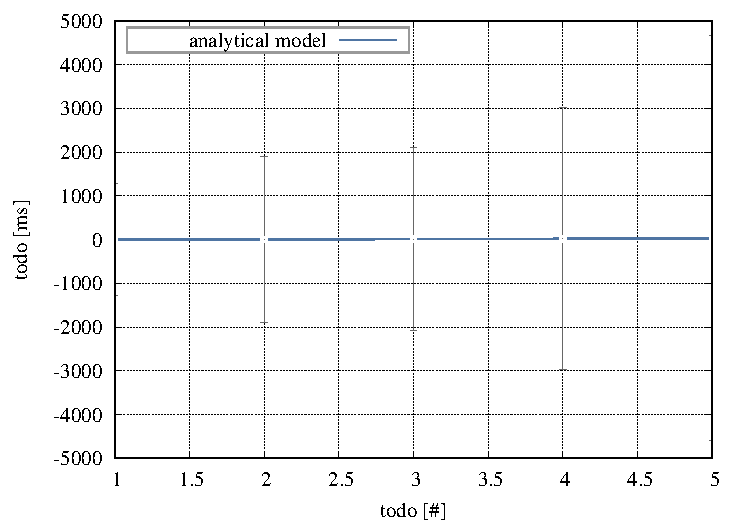
\includegraphics[width=.55\textwidth]{resources/images/example1}
    \caption{Example (based on~\cite{li2002design})}\label{fig:intro:a}
\end{figure}

\sidenote{Application Area: Foo Fooli}\index{Foo!Fooli}
\todomid{write about the application area~\cite{Heflin2004}}

\begin{figure}[H]
      \centering
      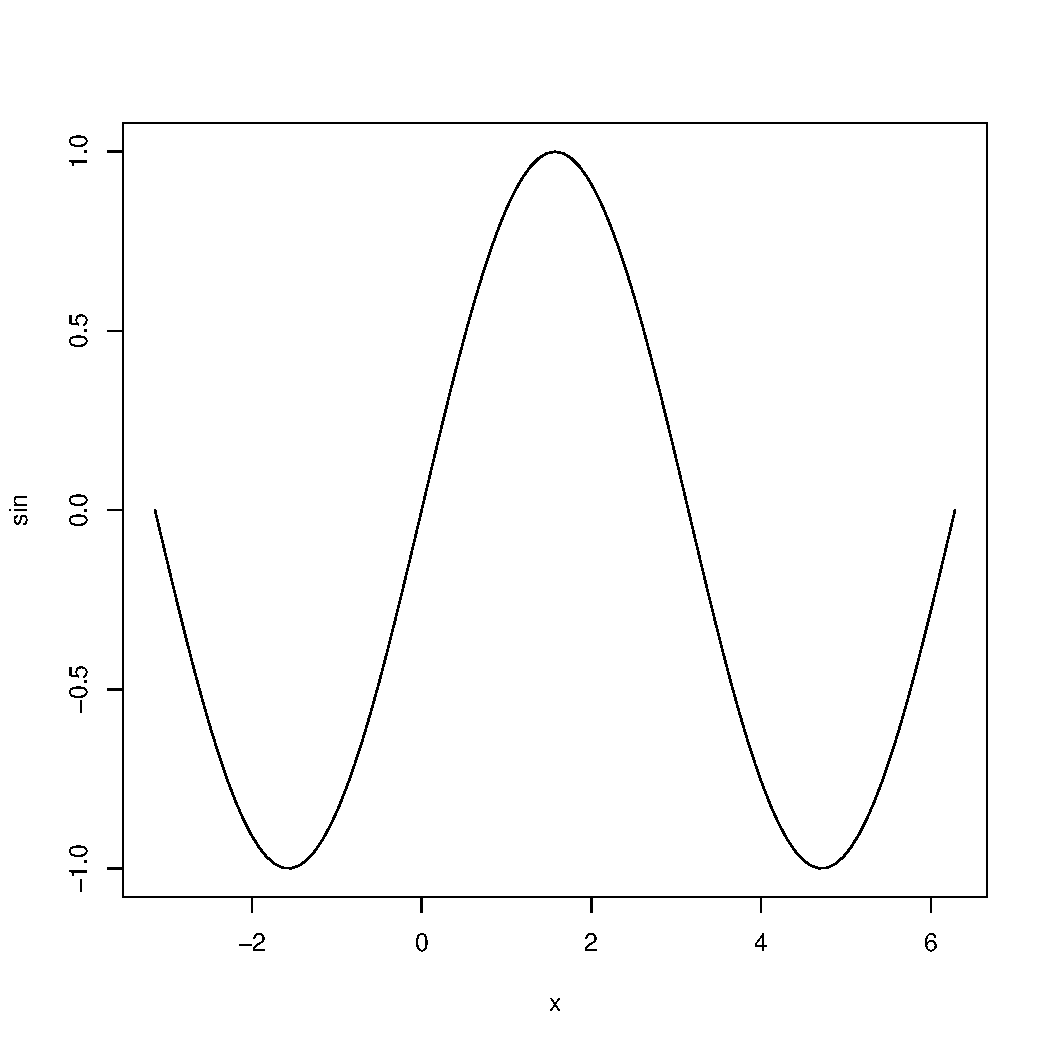
\includegraphics[width=.45\textwidth]{resources/images/example2}
      \caption{Another example~\cite{li2002design}}\label{fig:intro:b}
\end{figure}

\sidenote{Research Focus: Bar Barli}\index{Bar!Barli}
\todomid{write about the research focus and \Cref{fig:intro:b}}

\sidenote{Taxonomy}\index{Taxonomy}
\todomid{write about the taxonomy and \ac{ABAC}}

\begin{figure}[htbp]
      \centering
      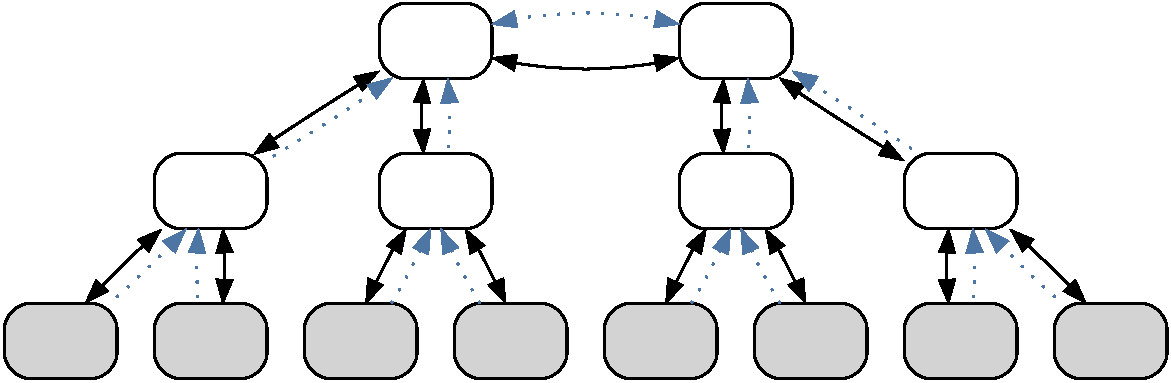
\includegraphics[width=.75\textwidth]{resources/images/example3}
      \caption{Taxonomy}
\end{figure}

\section{Problem Statement}\index{Requirements}

\sidenote{State of the Art}
\todomid{write about the State of the Art}

\sidenote{Issue:\\Example 1}
\todomid{write about the first issue}

\sidenote{Issue:\\Example 2}
\todomid{write about the second issue}

\sidenote{Synopsis}
\todomid{write about the synopsis of the issues and \Cref{fig:intro:c}}

\begin{figure}[htbp]
    \centering
    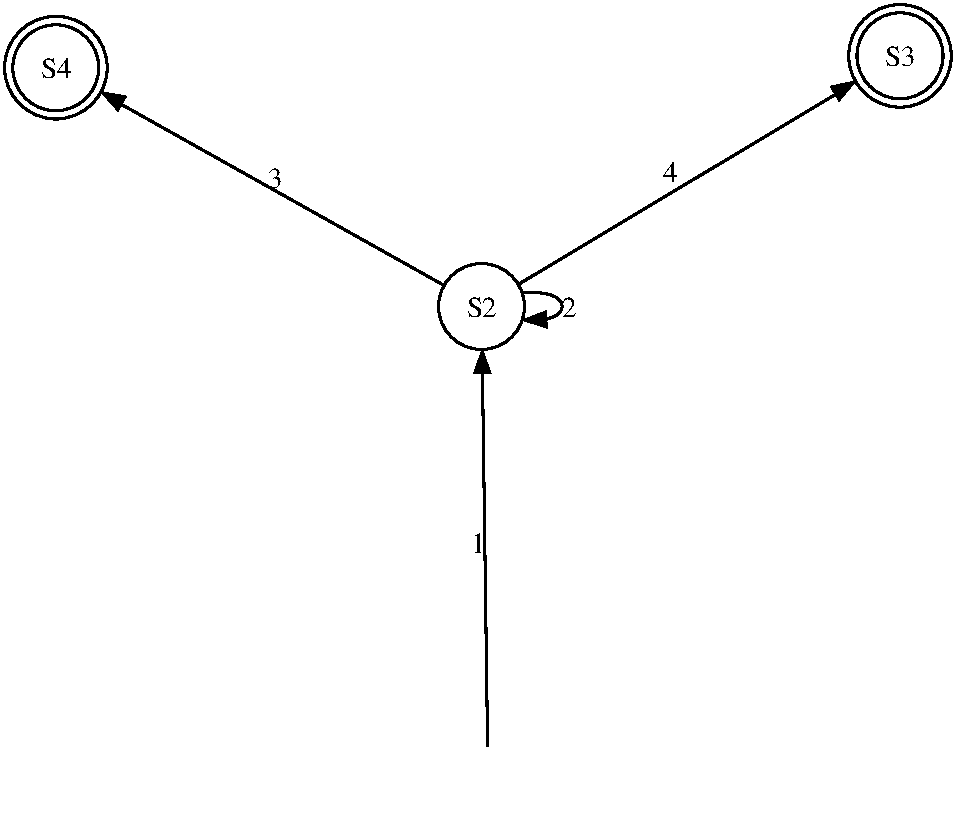
\includegraphics[width=.5\textwidth]{resources/images/job_lifecycle}
    \caption{Relationship between issues}\label{fig:intro:c}
\end{figure}

\section{Assumptions and Scope}

\sidenote{Research Assumptions}
\todomid{write about the research assumptions~\cite{li2002design}}

\sidenote{Research Scope}
\todomid{write about the research scope --- \Cref{fig:intro:a,fig:intro:b,fig:intro:c}}


\section{Objectives and Contributions}

\begin{figure}[htbp]
    \centering
    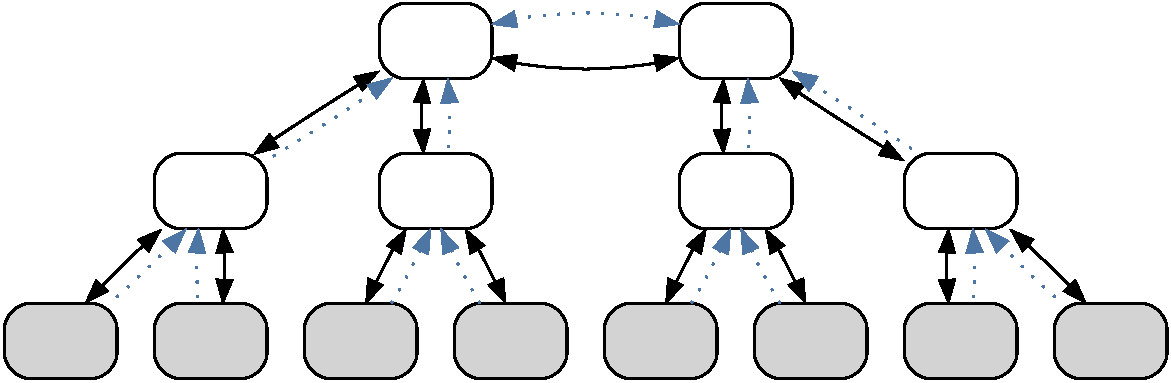
\includegraphics[width=.55\textwidth]{resources/images/example3}
    \caption{Structure of research}\label{fig:intro:struct}
\end{figure}

\sidenote{Research Objectives \& Contributions}
\todomid{write about the research objectives and \ac{DBpedia} and \Cref{fig:intro:struct}}

\section{Methodology and Outline}

\todomid{write about the research outline and \Cref{fig:intro:methodology}. Summarize \Cref{sec:introduction,sec:sota,sec:reqs,sec:contrib1,sec:contrib2,sec:contrib3,sec:eval,sec:summary}.}

\begin{sidewaysfigure}
    \centering
    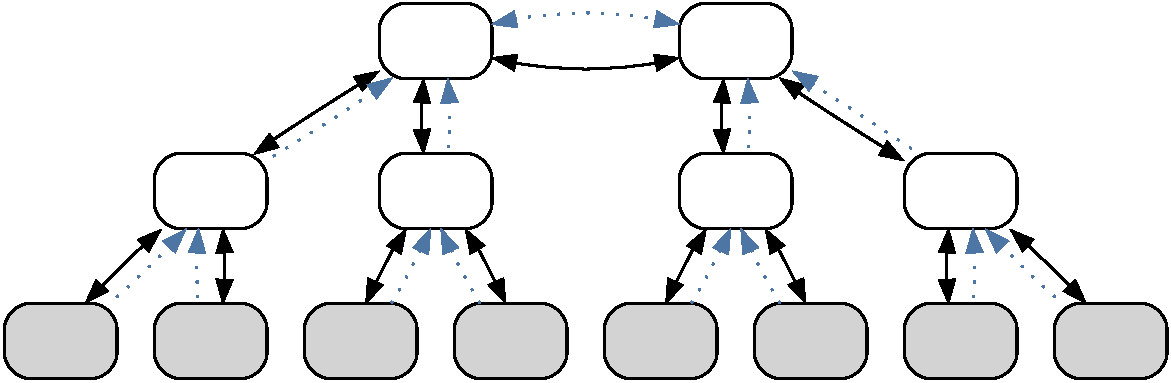
\includegraphics[width=.7\textwidth]{resources/images/example3}
    \caption{Workflow of the research and structure of the thesis}\label{fig:intro:methodology}
\end{sidewaysfigure}

    \cleardoublepage\chapter{State of the Art}\label{sec:sota}\minitoc\vspace{.5cm}\index{SotA}

\section{Introduction}

\begin{wrapfigure}{r}{0.2\textwidth}
    \centering
    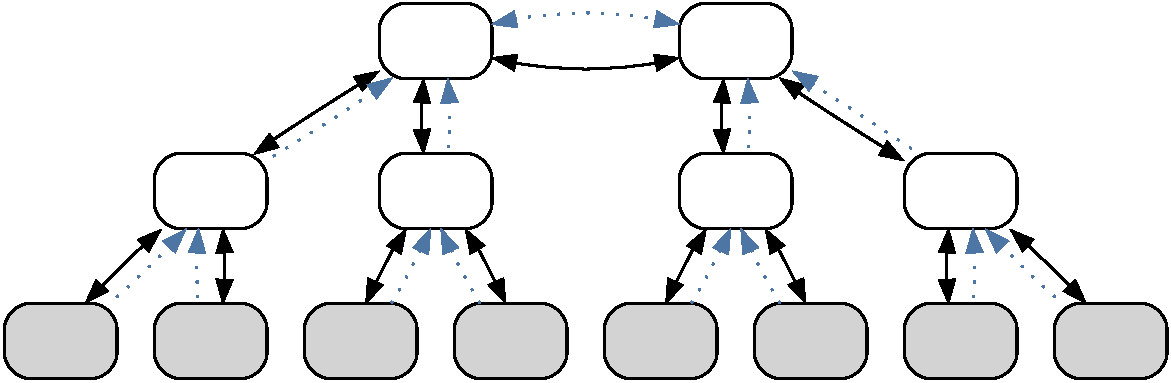
\includegraphics[width=0.2\textwidth]{resources/images/example3}
\end{wrapfigure}

\sidenote{Overview}
\todomid{write}

\section{Related Area 1}\index{Related Area}

\begin{figure}[H]
    \centering
    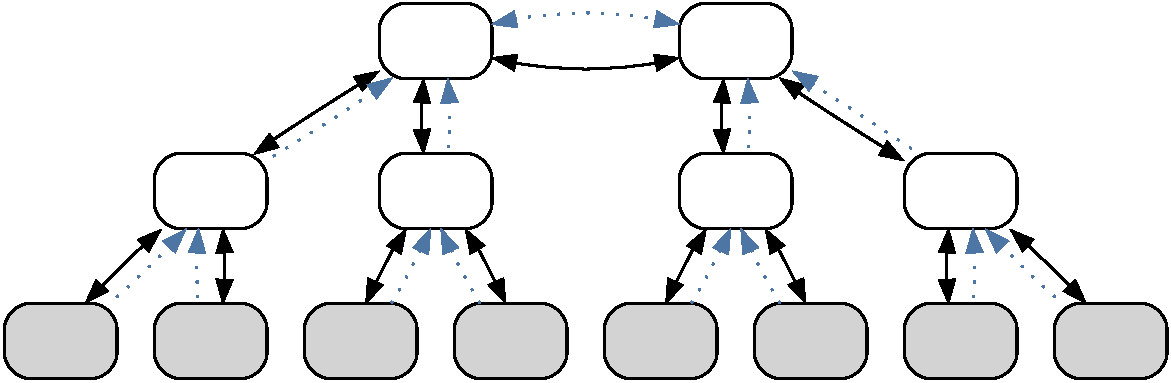
\includegraphics[width=.55\textwidth]{resources/images/example3}
    \caption{Related area 1 within the structure of research}\label{fig:hourglass:ra1}
\end{figure}

\sidenote{Overview}
\todomid{write about \Cref{fig:hourglass:ra1}}

\sidenote{Focus}
oder auch Abkürzungen wie \ac{ab} und \ac{dae}.

\subsection{Specific Example 1}

\sidenote{Definition}
\todomid{write}

\sidenote{Issues}
\todomid{write}

\subsection{Specific Example 2}

\sidenote{Definition}
Irgendein Text mit acronymen \ac{ABAC}	\autocite{Auer2007}, oder \ac{sundials} oder \ac{DBpedia} \cite{li2002design,Yuan2005}

\sidenote{Implementations}
\todomid{write}

\sidenote{Research}
Wiederhole ein zwei Abkürzungen wie \ac{sundials} oder \ac{DBpedia}


\sidenote{Standards}
\todomid{write}

\sidenote{Adoption}
\todomid{write}

\subsection{Specific Example 3}\index{Example 3}

\sidenote{Transition}
\todomid{write about \Cref{fig:sota:trans}}

\begin{figure}
    \centering
    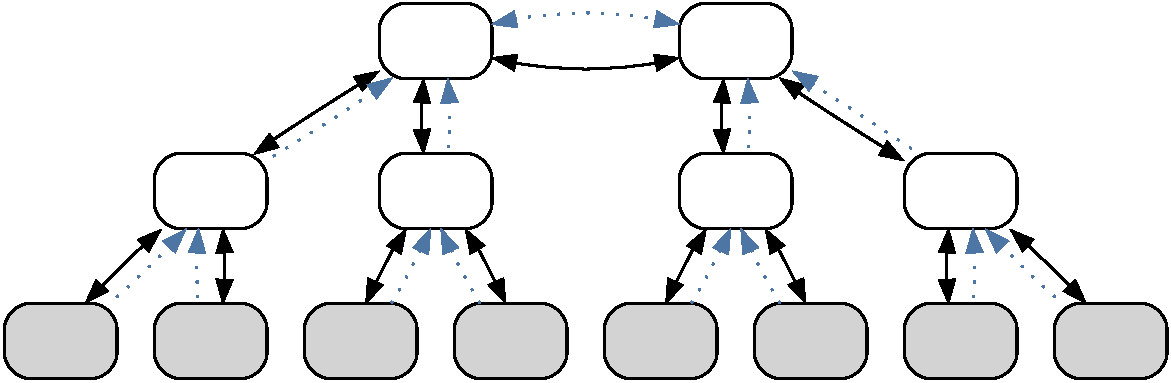
\includegraphics[width=.85\textwidth]{resources/images/example3}
    \caption{Comparison of Example 2 and Example 3 (based on~\cite{li2002design})}\label{fig:sota:trans}
\end{figure}

\sidenote{Standards}
\todomid{write}

\sidenote{Extension}
\todomid{write}

\sidenote{Other Standards}
\todomid{write}

\sidenote{Something}
\todomid{write}

\sidenote{Something}
\todomid{write}

\sidenote{Something}
\todomid{write}

\sidenote{Something}
\todomid{write}

\sidenote{Something}
\todomid{write}

\sidenote{Something}
\todomid{write}

\section{Related Area 2}\index{Related Area 2}

\sidenote{Overview}
\todomid{write}

\sidenote{Focus}
\todomid{write about \Cref{fig:sota:ra2}}

\begin{figure}[!hbtp]
    \centering
    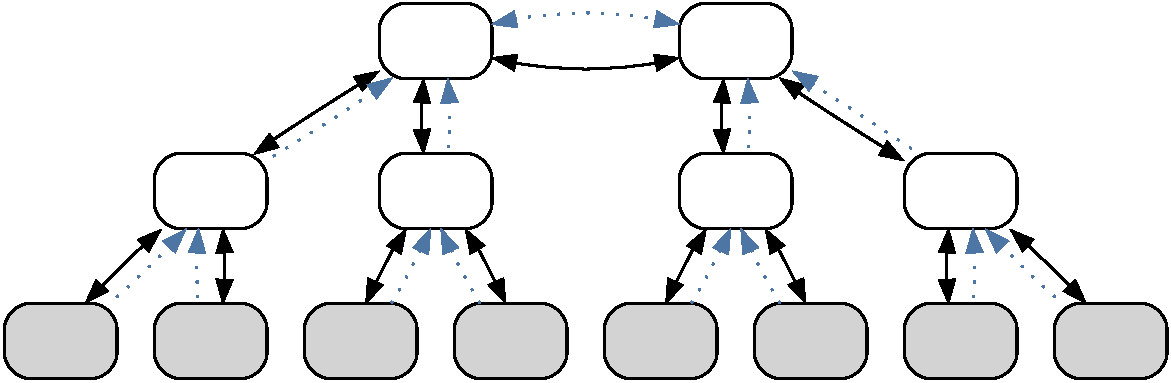
\includegraphics[width=1\textwidth]{resources/images/example3}
    \caption{Related Area 2}\label{fig:sota:ra2}
\end{figure}

\sidenote{Something}
\todomid{write}

\subsection{Specific Example 1}

\sidenote{Definition}
\todomid{write}

\sidenote{Issues}
\todomid{write}

\subsection{Specific Example 2}

\sidenote{Definition}
\todomid{write}

\sidenote{Implementations}
\todomid{write}

\sidenote{Research}
\todomid{write}

\sidenote{Standards}
\todomid{write}

\sidenote{Adoption}
\todomid{write}


\section{Related Area 3}\index{Related Area 3}

\sidenote{Overview}
\todomid{write}

\sidenote{Focus}
\todomid{write about \Cref{fig:sota:ra3}}

\begin{figure}[!hbtp]
    \centering
    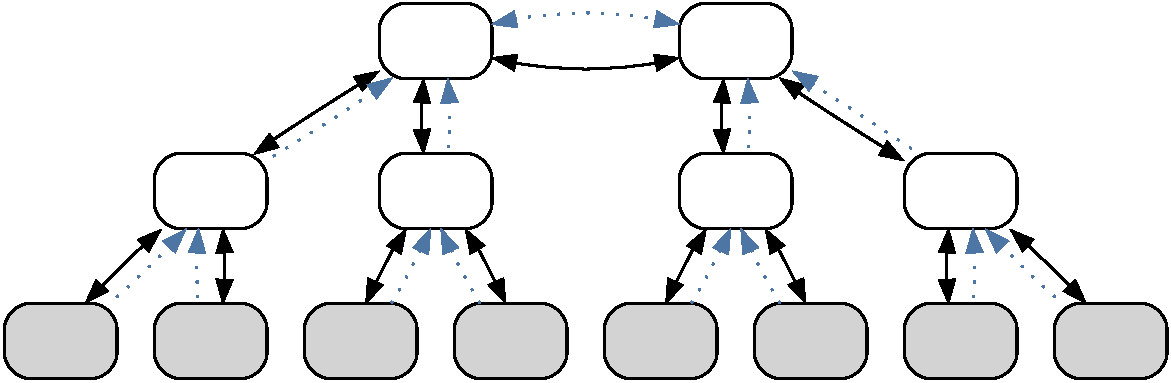
\includegraphics[width=1\textwidth]{resources/images/example3}
    \caption{Related Area 3}\label{fig:sota:ra3}
\end{figure}

\sidenote{Something}
\todomid{write}

\subsection{Specific Example 1}

\sidenote{Definition}
\todomid{write}

\sidenote{Issues}
\todomid{write}

\subsection{Specific Example 2}

\sidenote{Definition}
\todomid{write}

\sidenote{Implementations}
\todomid{write}

\sidenote{Research}
\todomid{write}

\sidenote{Standards}
\todomid{write}

\sidenote{Adoption}
\todomid{write}

\section{Conclusion}

\sidenote{Summary}
\todomid{write}

\sidenote{Takeaway 1}
\todomid{write}

\sidenote{Takeaway 2}
\todomid{write}

\sidenote{Takeaway 3}
\todomid{write}

\sidenote{Next chapter}
\todomid{write}

    \input{src/03_requirements}
    \input{src/04_contrib1}
    \input{src/05_contrib2}
    \input{src/06_contrib3}
    \input{src/07_evaluation}
    \input{src/08_summary}
    \nolinenumbers
    \cleardoublepage

    \appendix
    \pagenumbering{Roman}
    \setcounter{page}{1}
    \input{src/09_appendix}

    \cleardoublepage
    %\cleardoublepage
%\stepcounter{chapter}
%\renewcommand{\glossaryname}{Glossary}
%\markboth{\glossaryname}{\glossaryname}
%\renewcommand*{\chapterthumbformat}{\glossaryname}
%\printglossary%

\cleardoublepage
\chapter*{Bibliography}
\mtcaddchapter\addstarredchapter{Bibliography}
\markboth{Bibliography}{Bibliography}
\stepcounter{chapter}
%\renewcommand*{\chapterthumbformat}{Bibliography}
%\minitoc\vspace{.5cm}


\defbibfilter{papers}{
  type=article
  or type=inproceedings
  or type=proceedings
  or type=journal
  or type=phdthesis
  or type=incollection
  or type=book
  or keyword=thesis
  and not keyword=W3C
  and not keyword=RFC
  and not keyword=ITU
  and not keyword=IEEE
  and not keyword=ANSI
  and not keyword=OGF
  and not keyword=web
   and not keyword=online
  and not keyword=presentation
  and not keyword=workingpaper
}
\newrefcontext[labelprefix=p]
\printbibliography[filter=papers,heading=subbibliography,category=cited,title={References to Scientific Publications}]
%---
\defbibfilter{online}{
  type=online
  or type=web
  or type=www
}
\newrefcontext[labelprefix=o]
\printbibliography[filter=online,heading=subbibliography,category=cited,title={Online References}]
%---
\defbibfilter{standard}{
  type=techreport
  or type=report
  or keyword=W3C
  or keyword=RFC
  or keyword=TMF
  or keyword=ITU
  or keyword=IEEE
  or keyword=ANSI
  or keyword=OGF
  or keyword=ETSI
  or keyword=OneM2M
  or keyword=IETF
  or keyword=OMA
  or keyword=TMG
  or keyword=NIST
  or keyword=SNIA
  or keyword=OMG
  or keyword=DMTF
  or keyword=OASIS
  or keyword=deliverable
  or keyword=techreport
  or keyword=whitepaper
  and not keyword=web
  and not keyword=online
  and not keyword=presentation
  and not keyword=workingpaper
}
\newrefcontext[labelprefix=t]
\printbibliography[heading=subbibliography,filter=standard,category=cited,title={Technical References}]
%------------------
\defbibfilter{misc}{
  keyword=web
  or keyword=presentation
  or keyword=workingpaper
}
\newrefcontext[labelprefix=m]
\printbibliography[heading=subbibliography,filter=misc,category=cited,title={Miscellaneous References}]

%------
\nocite{*}
\newrefcontext[labelprefix=x]
\printbibliography[heading=subbibliography,notcategory=cited,title={Not referenced (will be empty)}]


    \backmatter
    \cleardoublepage\cleardoublepage
%\phantomsection
%\chapter{Index}
%\stepcounter{chapter}
%\renewcommand{\indexname}{Index}
%\renewcommand*{\chapterthumbformat}{\indexname}
%\markboth{\indexname}{\indexname}
\printindex

\end{document}
% ------------------------------------------------------------------------------

%%% Only for koma script
%\subject{\metaSubject}
%\title{\metaTitle}
%\author{\metaAuthor}
%\date{\metaDate}
%\dedication{\metaDedication}

\hypersetup{
      pdfauthor={\metaAuthorShort~<\metaAuthorMail>},
      pdfsubject={\metaSubject},
      pdftitle={\metaTitle},
      pdfkeywords={\metaKeywords},
      pdfcreator={http://github.com/tubav/},
      pdfproducer={pdfTeX},
      pdfpagelayout=TwoPageRight
}

% ------------------------------------------------------------------------------


% final fixes ------------------------------------------------------------------
\righthyphenmin=2
\tolerance=2000
\emergencystretch=10pt
% ------------------------------------------------------------------------------

% PDF/A color profile ----------------------------------------------------------
\immediate\pdfobj stream attr{/N 3}  file{lib/resources/pdfa/srgb.icc}% chktex 1
\pdfcatalog{%
/OutputIntents [ <<
/Type /OutputIntent
/S/GTS_PDFA1
/DestOutputProfile \the\pdflastobj\space 0 R
/OutputConditionIdentifier (sRGB IEC61966-2.1)% chktex 8
/Info(sRGB IEC61966-2.1)% chktex 8 chktex 36
>> ]
}
% ------------------------------------------------------------------------------
